\documentclass[convert={density=300,size=1080x800,outext=.png}]{standalone}

\usepackage[latin1]{inputenc}
\usepackage{tikz}

\usetikzlibrary{shapes,arrows,calc,fit,positioning}
\begin{document}
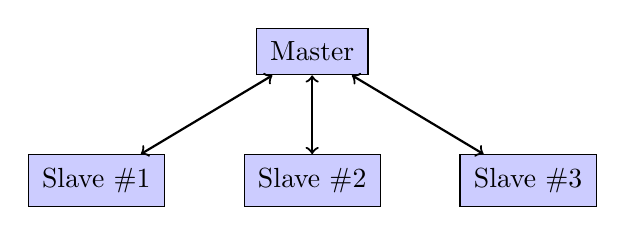
\begin{tikzpicture}[
  outer/.style={inner sep=5pt},
  block/.style={rectangle, draw, fill=blue!20}
  ]
  \node[outer, block] (A) {Master};
  \node[outer, block, below=of A] (C) {Slave \#2};
  \node[outer, block, left=of C] (B) {Slave \#1};
  \node[outer, block, right=of C] (D) {Slave \#3};

  \draw[thick,black,<->] (A) -- (C);
  \draw[thick,black,<->] (A) -- (B);
  \draw[thick,black,<->] (A) -- (D);
\end{tikzpicture}

\end{document}